\section{Gates}
\subsection{AND}
\begin{center}
    \begin{minipage}{0.55\linewidth}
        \begin{equation*}
            Y = A \land B \quad Y = A \cdot B
        \end{equation*}
        \begin{center}
            \begin{tikzpicture}[circuit logic IEC]
                \node[and gate] (and) at (0,0) {};
                \node[] (iA) at (-1, 0.4) {A};
                \node[] (iB) at (-1, -0.4) {B};
                \node[] (oZ) at (1, 0) {Y};
                \draw (iA.east) --++ (right:2mm) |- (and.input 1);
                \draw (iB.east) --++ (right:2mm) |- (and.input 2);
                \draw (and.output) -- (oZ);
            \end{tikzpicture}
        \end{center}
    \end{minipage}
    \hfill
    \begin{minipage}{0.35\linewidth}
        \begin{tabular}{|c c|c|}
            \hline
            A & B & Y\\
            \hline
            0 & 0 & 0\\
            0 & 1 & 0\\
            1 & 0 & 0\\
            1 & 1 & 1\\
            \hline
        \end{tabular}
    \end{minipage}
    \begin{minipage}[t]{0.45\linewidth}
        \subsubsection{NAND}
        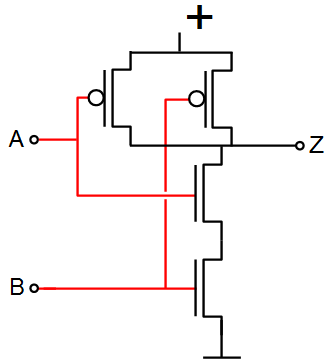
\includegraphics[width = 30mm]{images/nand.png}
    \end{minipage}
    \begin{minipage}[t]{0.45\linewidth}
        \subsubsection{AND aus NOR}
        \begin{adjustbox}{width = 30mm}
            \begin{tikzpicture}[circuit logic IEC]
                \matrix[column sep=5mm]{
                    \node[] (iA) {A}; & \node[nor gate] (nor1) {}; & &\\
                    & & \node[nor gate] (nor3) {}; & \node[] (oZ) {Y};\\
                    \node[] (iB) {B}; & \node[nor gate] (nor2) {}; & &\\
                };
                \draw (iA.east) --++(right:2.5mm) |- (nor1.input 1);
                \draw (iA.east) --++(right:2.5mm) |- (nor1.input 2);
                \draw (iB.east) --++(right:2.5mm) |- (nor2.input 1);
                \draw (iB.east) --++(right:2.5mm) |- (nor2.input 2);
                \draw (nor1.output) --++(right:2.5mm) |- (nor3.input 1);
                \draw (nor2.output) --++(right:2.5mm) |- (nor3.input 2);
                \draw (nor3.output) -- (oZ);
            \end{tikzpicture}
        \end{adjustbox}
    \end{minipage}
\end{center}

\subsection{OR}
\begin{center}
    \begin{minipage}{0.55\linewidth}
        \begin{equation*}
            Y = A \lor B \quad Y = A + B
        \end{equation*}
        \begin{center}
            \begin{tikzpicture}[circuit logic IEC]
                \node[or gate] (or) at (0,0) {};
                \node[] (iA) at (-1, 0.4) {A};
                \node[] (iB) at (-1, -0.4) {B};
                \node[] (oZ) at (1, 0) {Y};
                \draw (iA.east) --++ (right:2mm) |- (or.input 1);
                \draw (iB.east) --++ (right:2mm) |- (or.input 2);
                \draw (or.output) -- (oZ);
            \end{tikzpicture}
        \end{center}
    \end{minipage}
    \hfill
    \begin{minipage}{0.35\linewidth}
        \begin{tabular}{|c c|c|}
            \hline
            A & B & Y\\
            \hline
            0 & 0 & 0\\
            0 & 1 & 1\\
            1 & 0 & 1\\
            1 & 1 & 1\\
            \hline
        \end{tabular}
    \end{minipage}
    \begin{minipage}[t]{0.45\linewidth}
        \subsubsection{NOR}
        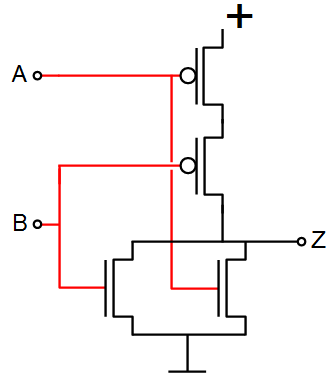
\includegraphics[width = 30mm]{images/nor.png}
    \end{minipage}
    \begin{minipage}[t]{0.45\linewidth}
        \subsubsection{OR aus NAND}
        \begin{adjustbox}{width = 30mm}
            \begin{tikzpicture}[circuit logic IEC]
                \matrix[column sep=5mm]{
                    \node[] (iA) {A}; & \node[nand gate] (nand1) {}; & &\\
                    & & \node[nand gate] (nand3) {}; & \node[] (oZ) {Y};\\
                    \node[] (iB) {B}; & \node[nand gate] (nand2) {}; & &\\
                };
                \draw (iA.east) --++(right:2.5mm) |- (nand1.input 1);
                \draw (iA.east) --++(right:2.5mm) |- (nand1.input 2);
                \draw (iB.east) --++(right:2.5mm) |- (nand2.input 1);
                \draw (iB.east) --++(right:2.5mm) |- (nand2.input 2);
                \draw (nand1.output) --++(right:2.5mm) |- (nand3.input 1);
                \draw (nand2.output) --++(right:2.5mm) |- (nand3.input 2);
                \draw (nand3.output) -- (oZ);
            \end{tikzpicture}
        \end{adjustbox}
    \end{minipage}
\end{center}

\subsection{NOT}
\begin{center}
    \begin{minipage}{0.3\linewidth}
        \begin{equation*}
            Y = \overline{A}
        \end{equation*}
        \begin{center}
            \begin{tikzpicture}[circuit logic IEC]
                \node[not gate] (not) at (0,0) {};
                \node[] (iA) at (-0.8, 0) {A};
                \node[] (oZ) at (0.8, 0) {Y};
                \draw (iA.east) -- (not.input);
                \draw (not.output) -- (oZ);
            \end{tikzpicture}
        \end{center}
    \end{minipage}
    \hfill
    \begin{minipage}{0.2\linewidth}
        \begin{tabular}{|c|c|}
            \hline
            A & Y \\
            0 & 1\\
            1 & 0\\
            \hline
        \end{tabular}
    \end{minipage}
    \hfill
    \begin{minipage}{0.3\linewidth}
        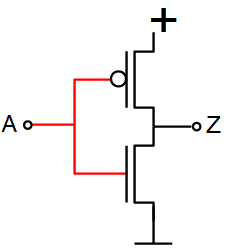
\includegraphics[width = 20mm]{images/not.png}
    \end{minipage}
    \begin{minipage}{0.45\linewidth}
        \subsubsection{NOT aus NOR}
        \begin{center}
            \begin{tikzpicture}[circuit logic IEC]
            \node[nor gate] (gate) at (0,0) {};
            \node[] (iA) at (-1, 0) {A};
            \node[] (oZ) at (1, 0) {Y};
            \draw (iA.east) --++ (right:2mm) |- (gate.input 1);
            \draw (iA.east) --++ (right:2mm) |- (gate.input 2);
            \draw (gate.output) -- (oZ);
            \end{tikzpicture}
        \end{center}
    \end{minipage}
    \hfill
    \begin{minipage}{0.45\linewidth}
        \subsubsection{NOT aus NAND}
        \begin{center}
            \begin{tikzpicture}[circuit logic IEC]
            \node[nand gate] (gate) at (0,0) {};
            \node[] (iA) at (-1, 0) {A};
            \node[] (oZ) at (1, 0) {Y};
            \draw (iA.east) --++ (right:2mm) |- (gate.input 1);
            \draw (iA.east) --++ (right:2mm) |- (gate.input 2);
            \draw (gate.output) -- (oZ);
            \end{tikzpicture}
        \end{center}
    \end{minipage}
\end{center}

\subsection{Weitere Gates}
\begin{center}
    \begin{minipage}{0.21\linewidth}
        \subsubsection{NAND}
        \begin{equation*}
            C = \overline{A \land B}
        \end{equation*}
        \begin{center}
            \begin{adjustbox}{width = 14mm}
                \begin{tikzpicture}[circuit logic IEC, thick]
                    \node[nand gate] (nand) at (0,0) {};
                    \node[] (iA) at (-0.8, 0.4) {A};
                    \node[] (iB) at (-0.8, -0.4) {B};
                    \node[] (oZ) at (0.8, 0) {C};
                    \draw (iA.east) --++ (right:1.5mm) |- (nand.input 1);
                    \draw (iB.east) --++ (right:1.5mm) |- (nand.input 2);
                    \draw (nand.output) -- (oZ);
                \end{tikzpicture}
            \end{adjustbox}
        \end{center}
    \end{minipage}
    \hfill\vline\hfill
    \begin{minipage}{0.21\linewidth}
        \subsubsection{NOR}
        \begin{equation*}
            D = \overline{A \lor B}
        \end{equation*}
        \begin{center}
            \begin{adjustbox}{width = 14mm}
                \begin{tikzpicture}[circuit logic IEC, thick]
                    \node[nor gate] (nor) at (0,0) {};
                    \node[] (iA) at (-0.8, 0.4) {A};
                    \node[] (iB) at (-0.8, -0.4) {B};
                    \node[] (oZ) at (0.8, 0) {D};
                    \draw (iA.east) --++ (right:1.5mm) |- (nor.input 1);
                    \draw (iB.east) --++ (right:1.5mm) |- (nor.input 2);
                    \draw (nor.output) -- (oZ);
                \end{tikzpicture}
            \end{adjustbox}
        \end{center}
    \end{minipage}
    \hfill\vline\hfill
    \begin{minipage}{0.21\linewidth}
        \subsubsection{XNOR}
        \begin{equation*}
            E = \overline{A \oplus B}
        \end{equation*}
        \begin{center}
            \begin{adjustbox}{width = 14mm}
                \begin{tikzpicture}[circuit logic IEC, thick]
                    \node[xnor gate] (xnor) at (0,0) {};
                    \node[] (iA) at (-0.8, 0.4) {A};
                    \node[] (iB) at (-0.8, -0.4) {B};
                    \node[] (oZ) at (0.8, 0) {E};
                    \draw (iA.east) --++ (right:1.5mm) |- (xnor.input 1);
                    \draw (iB.east) --++ (right:1.5mm) |- (xnor.input 2);
                    \draw (xnor.output) -- (oZ);
                \end{tikzpicture}
            \end{adjustbox}
        \end{center}
    \end{minipage}
    \hfill\vline\hfill
    \begin{minipage}{0.21\linewidth}
        \subsubsection{XOR}
        \begin{equation*}
            F = A \oplus B
        \end{equation*}
        \begin{center}
            \begin{adjustbox}{width = 14mm}
                \begin{tikzpicture}[circuit logic IEC, thick]
                    \node[xor gate] (xor) at (0,0) {};
                    \node[] (iA) at (-0.8, 0.4) {A};
                    \node[] (iB) at (-0.8, -0.4) {B};
                    \node[] (oZ) at (0.8, 0) {F};
                    \draw (iA.east) --++ (right:1.5mm) |- (xor.input 1);
                    \draw (iB.east) --++ (right:1.5mm) |- (xor.input 2);
                    \draw (xor.output) -- (oZ);
                \end{tikzpicture}
            \end{adjustbox}
        \end{center}
    \end{minipage}
\end{center}
\begin{center}
    \begin{tabular}{|c c|c|c|c|c|}
        \hline
        & & \rotatebox{90}{\tiny NAND} & \rotatebox{90}{\tiny NOR}& \rotatebox{90}{\tiny XNOR} & \rotatebox{90}{\tiny XOR}\\
        A & B & C & D & E & F\\
        \hline
        0 & 0 & 1 & 1 & 1 & 0\\
        0 & 1 & 1 & 0 & 0 & 1\\
        1 & 0 & 1 & 0 & 0 & 1\\
        1 & 1 & 0 & 0 & 1 & 0\\
        \hline
    \end{tabular}
\end{center}
\subsubsection{XOR aus NAND}
\begin{center}
    \begin{minipage}{0.45\linewidth}
        \begin{adjustbox}{width = 30mm}
            \begin{tikzpicture}[circuit logic IEC, thick]
                \matrix[column sep=5mm]{
                    \node[] (iA) {A}; & & \node[nand gate] (upperNand) {}; & \\
                    & \node[nand gate] (mNand1) {}; & & \node[nand gate] (mNand2) {}; & \node[] (oF) {F};\\
                    \node[] (iB) {B}; & & \node[nand gate] (lowerNand) {}; & \\
                };
                \draw[] (iA) --++ (right:10mm) |- (upperNand.input 1);
                \draw[] (iB) --++ (right:10mm) |- (lowerNand.input 2);
                \draw[] (iA) --++ (right:5mm) |- (mNand1.input 1);
                \draw[] (iB) --++ (right:5mm) |- (mNand1.input 2);
                \draw[] (mNand1.output) --++ (right:2.5mm) |- (upperNand.input 2);
                \draw[] (mNand1.output) --++ (right:2.5mm) |- (lowerNand.input 1);
                \draw[] (upperNand.output) --++ (right:2.5mm) |- (mNand2.input 1);
                \draw[] (lowerNand.output) --++ (right:2.5mm) |- (mNand2.input 2);
                \draw[] (mNand2.output) -- (oF);
                \node[right = 2.4mm of iA, circ] {}; 
                \node[right = 2.4mm of iB, circ] {}; 
                \node[right = 2mm of mNand1.output, circ] {}; 
            \end{tikzpicture}
        \end{adjustbox}
    \end{minipage}
    \begin{minipage}{0.45\linewidth}
        \textbf{XOR aus NOR:} Gleiches Schema wie NAND + 1 Inverter\\
        \vspace{-2mm}\hrule\vspace{1mm}
        \textbf{XNOR aus NAND:} Gleiches Schema wie \textit{XOR aus NOR}\\
        \vspace{-2mm}\hrule\vspace{1mm}
        \textbf{XNOR aus NOR:} Gleiches Schema wie \textit{XOR aus NAND}\\
    \end{minipage}
\end{center}
{\tiny Es versteht sich natürlich, dass wenn von \glqq Gleichem Schema wie\dots\grqq{} gesprochen wird, die Gates trotzdem getauscht werden müssen.}
